%
% File acl2015.tex
%
% Contact: car@ir.hit.edu.cn, gdzhou@suda.edu.cn
%%
%% Based on the style files for ACL-2014, which were, in turn,
%% Based on the style files for ACL-2013, which were, in turn,
%% Based on the style files for ACL-2012, which were, in turn,
%% based on the style files for ACL-2011, which were, in turn, 
%% based on the style files for ACL-2010, which were, in turn, 
%% based on the style files for ACL-IJCNLP-2009, which were, in turn,
%% based on the style files for EACL-2009 and IJCNLP-2008...

%% Based on the style files for EACL 2006 by 
%%e.agirre@ehu.es or Sergi.Balari@uab.es
%% and that of ACL 08 by Joakim Nivre and Noah Smith

\documentclass[11pt]{article}
\usepackage{acl2015}
\usepackage{times}
\usepackage{url}
\usepackage{latexsym}
\usepackage[utf8]{inputenc}
\usepackage{hyperref}
\usepackage[table]{xcolor}
\usepackage{graphicx}
%\setlength\titlebox{5cm}

% You can expand the titlebox if you need extra space
% to show all the authors. Please do not make the titlebox
% smaller than 5cm (the original size); we will check this
% in the camera-ready version and ask you to change it back.


\title{Inmon vs Kimball}

\author{First Author \\
Esperilla Ruiz Adnner \\
  {\tt email@domain} \\}

\date{}

\begin{document}
\maketitle
\begin{abstract}
    \input{resumen}
\end{abstract}


\section{Introduction}


\section{Objetivos}
\begin{enumerate}
    \item Determinar la diferencia entre las dos perspectivas presentadas.
\end{enumerate}


\section{Marco Teórico}

\subsection{El enfoque de Inmon}

\begin{enumerate}
    \item \textbf{Orientado a temas:} Los datos en la base de datos están organizados de manera que todos los elementos de datos relativos al mismo evento u objeto del mundo real queden unidos entre sí.
    \item \textbf{Integrado:} La base de datos contiene los datos de todos los sistemas operacionales de la organización, y dichos datos deben ser consistentes. 
\item \textbf{No volátil:} La información no se modifica ni se elimina, una vez almacenado un dato, éste se convierte en información de sólo lectura, y se mantiene para futuras consultas.

\item \textbf{Variante en el tiempo} Los cambios producidos en los datos a lo largo del tiempo quedan registrados para que los informes que se puedan generar reflejen esas variaciones.

\end{enumerate}


\begin{figure}[htb]
\begin{center}
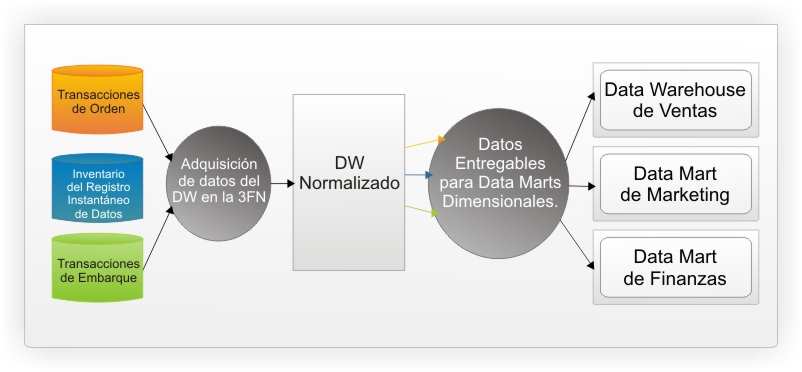
\includegraphics[width=8cm]{./images/enfoque-inmon.jpg}
\end{center}
\end{figure}

El enfoque Inmon tambien se referencia normalmente como Top-down. Los datos son extraidos de los sistemas operacionales por los procesos ETL y cargados en las areas de stage, donde son validados y consolidados en el DW corporativo, donde ademas existen los llamados metadatos que documentan de una forma clara y precisa el contenido del DW. Una vez realizado este proceso, los procesos de refresco de los Data Mart departamentales obtienen la información de el, y con las consiguientes transformaciones, organizan los datos en las estructuras particulares requeridas por cada uno de ellos, refrescando su contenido.\\


La metodologia para la construcción de un sistema de este tipo es la habitual para construir un sistema de información, utilizando las herramientas habituales (esquema Entidad Relacion, DIS (Data Item Sets, etc). Para el tratamiento de los cambios en los datos, usa la Continue and Discrete Dimension Management (inserta fechas en los datos para determinar su validez para las Continue Dimension o bien mediante el concepto de snapshot o foto para las Discrete Dimension).

\subsection{El enfoque Ralph Kimball.}
El Data Warehouse es un conglomerado de todos los Data Marts dentro de una empresa, siendo una copia de los datos transaccionales estructurados de una forma especial para el analisis, de acuerdo al Modelo Dimensional (no normalizado), que incluye, como ya vimos, las dimensiones de análisis y sus atributos, su organización jerarquica, asi como los diferentes hechos de negocio que se quieren analizar.

\begin{figure}[htb]
\begin{center}
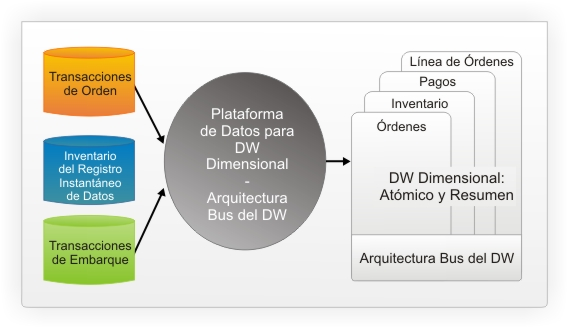
\includegraphics[width=8cm]{./images/enfoque-kimball.jpg}
\end{center}
\end{figure}


Los diferentes Data Marts estan conectados entre si por la llamada bus structure, que contiene los elementos anteriormente citados a traves de las dimensiones conformadas (que permiten que los usuarios puedan realizar querys conjuntos sobre los diferentes data marts, pues este bus contiene los elementos en común que los comunican).\\

La metodología para la construcción del Dw incluye las 4 fases que vimos en la entrada anterior del blog, que son: Selección del proceso de negocio, definición de la granuralidad de la información, elección de las dimensiones de análisis e identificación de los hechos o métricas. Igualmente define el tratamiento de los cambios en los datos a través de las Dimensiones Lentamente Cambiantes (SCD).



\section{Análisis}

{\bf ¿Cómo afectan estos factores a los dos modelos de datawarehouse? }

\large Factores
\begin{enumerate}
    \item Presupuesto
    \item Plazos
    \item Expertise
    \item Alcance
    \item Mantenimiento
\end{enumerate}

\large Inmon
\begin{enumerate}
    \item Coste inicial alto
    \item Requiere más tiempo de desarrollo
    \item Equipo con especialización alta
    \item Toda la compañía
    \item Fácil mantenimiento
\end{enumerate}

\large Kimball
\begin{enumerate}
    \item Coste inicial bajo
    \item Tiempo de desarrollo inferior
    \item Equipo con especialización media
    \item Departamentos individuales
    \item Mantenimiento más complejo
\end{enumerate}

\\Aparte de estas variables, que van a ser determinantes a la hora de decidirnos por un modelo u otro, tenemos que tener muy clara cuál será la finalidad de nuestro datawarehouse.

\section*{Conclusiones}

El datawarehouse de Kimball está orientado a la consulta de la información, por lo que su estructura interna está especialmente diseñada para garantizar una explotación de los datos rápida y sencilla, no requiriendo usuarios especializados para ello. Por el contrario, el datawarehouse de Inmon persigue la integración de todos los datos de la compañía, estando orientado hacia el almacenaje de grandes volúmenes de datos, por lo que su estructura interna normalizada se diseña para evitar la redundancia de datos, simplificar las labores de mantenimiento, etc. cuestiones que complican las consultas de la información, requiriendo que los usuarios finales estén mucho más especializados.
Así, podríamos decir que el enfoque de Kimball se ajusta más a proyectos pequeños en los que se persiga un sistema fácilmente explotable y entendible por el usuario y de rápido desarrollo, siendo el modelo de Inmon más apropiado para sistemas complejos de mayor envergadura.
Todo proyecto tiene sus propias peculiaridades, siendo cada caso único e independiente, por lo que resulta necesario llevar a cabo un estudio de todas ellas antes de decantarnos por una solución u otra, de forma que podamos hacernos una idea sobre qué modelo se ajusta mejor a las condiciones de nuestro proyecto.

% include your own bib file like this:
%\bibliographystyle{acl}
%\bibliography{acl2015}


\begin{thebibliography}{9}
    \bibitem{churriwifi} 
    churriwifi
    \textit{https://churriwifi.wordpress.com/2010/04/19/15-2-ampliacion-conceptos-del-modelado-dimensional/}. 
    

    \bibitem{bi-geek} 
    bi-geek\\
    \textit{https://blog.bi-geek.com/arquitectura-comparativa-inmon-y-kimball/}
    
    
    
    


\end{thebibliography}


\end{document}